% Title: Subset and equality constraints
% Author: Jakob Voß
%
% This diagram shows how OMR2 symbols for subset and equality constraints
% could be replaces by simple subtyping arrows.
\documentclass{article}
\usepackage{tkz-orm}
%\usetikzlibrary{positioning}
\begin{document}
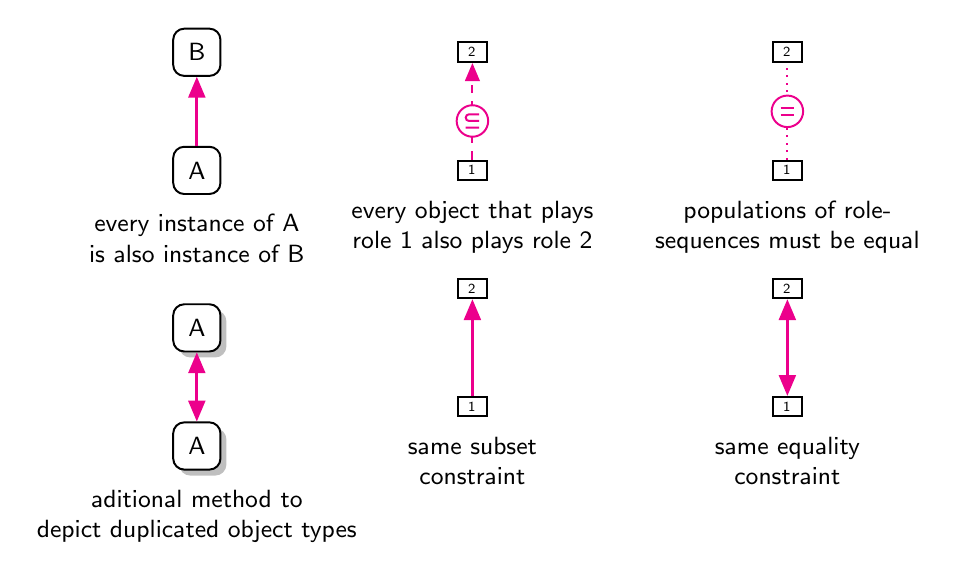
\begin{tikzpicture}[orm]
\entity (B) at (0,0) {B};
\entity[label={[align=center]below:every instance of A\\is also instance of B
}] (A) at (0,-1.5) {A};
\draw[subtype] (B) to (A);

\begin{scope}[xshift=3.5cm]
\unary[index=2] (a) at (0,0) {};
\unary[index=1,label={[align=center]below:
every object that plays\\role 1 also plays role 2
}] (b) at (0,-1.5) {};
\limitsto (b) to node[constraint=subset,pos=0.4]{} (a);
\end{scope}

\begin{scope}[yshift=-3.5cm]
\entity[duplicated] (B) at (0,0) {A};
\entity[duplicated,label={[align=center]below:aditional method to\\
depict duplicated object types}] (A) at (0,-1.5) {A};
\draw[subtype,<->] (B) to (A);
\end{scope}

\begin{scope}[xshift=7.5cm]
\unary[index=2] (a) at (0,0) {};
\unary[index=1,label={[align=center]below:
populations of role-\\sequences must be equal
}] (b) at (0,-1.5) {};
\limits (b) to node[constraint=equal]{} (a);
\end{scope}

\begin{scope}[xshift=3.5cm,yshift=-3cm]
\unary[index=2] (a) at (0,0) {};
\unary[index=1,label={[align=center]below:same subset\\constraint}] (b) at (0,-1.5) {};
\draw[subtype] (a) to (b);
\end{scope}

\begin{scope}[xshift=7.5cm,yshift=-3cm]]
\unary[index=2] (a) at (0,0) {};
\unary[index=1,label={[align=center]below:same equality\\constraint}] (b) at (0,-1.5) {};
\draw[subtype,<->] (b) to (a);
\end{scope}

\end{tikzpicture}
\end{document}